\documentclass{beamer}
%\documentclass[handout]{beamer}

% \usepackage{ensislidesOG}
%\usepackage[utf8]{inputenc}
% \usepackage[T1]{fontenc}
\usepackage[english]{babel}
\usepackage[sfdefault]{roboto} 
\usepackage{ulem}
\usepackage{amsfonts}
\usepackage{amsmath}
\usepackage{amssymb}
\usepackage{amsthm}
% \usepackage[frenchstyle]{mathalpha}
% \usepackage[OMLmathsfit]{isomath}
\usepackage{graphicx}
\usepackage{color} % for ps_tex inclusions
\usepackage{fmtcount} % th, e.g. \ordinalnum{4}
\usepackage{booktabs}

\usepackage{xr}
\usepackage{hyperref}
\externaldocument[notes-]{notes}

\usetheme{Madrid}
\usecolortheme{seagull}

\newcommand{\itb}{\item[$\bullet$]}
\newcommand{\dps}{\displaystyle}

\def\<{{\guillemotleft}}
\def\>{{\guillemotright}}

\def\vs1{\vspace{1mm}}
\def\v3{\vspace{3mm}}

\newcommand{\II}{\,\mbox{I\hskip -0.600em 1}}

\newcommand{\ME}{{\mathcal E}}
\newcommand{\MN}{{\mathcal N}}

\newcommand{\NN}{\ensuremath{\mathbb{N}}}
\newcommand{\RR}{\ensuremath{\mathbb{R}}}

\newcommand{\card}{\mbox{card}}
\newcommand{\pa}{\mbox{pa}}

\newcommand{\De}{\mbox{De}}
\newcommand{\Nd}{\mbox{Nd}}
\newcommand{\Ne}{\mbox{Ne}}

\newcommand{\indep}{\perp\!\!\!\perp}
\newcommand{\condindep}[3]{#1 \indep #2 \vert #3}
\newcommand{\condindepP}[4]{#1 \indep_{#4} #2 \vert #3}
\newcommand{\ts}[3]{#1_{#2}^{#3}}
\newcommand{\set}[1]{\{#1\}}
\newcommand{\bs}[1]{\boldsymbol{#1}}

\title{Learning Probabilities and Causality}

\subtitle{Chapter II - Gaussian mixture models (GMM) and the expectation-maximisation (EM) algorithm} % (optional)

\author[Xavi and Thomas]{Xavier Alameda-Pineda and Thomas Hueber}

\institute{Ensimag/Inria/CNRS/Univ. Grenoble-Alpes}


\makeatother
\setbeamertemplate{footline}
{
  \leavevmode%
%   \hbox{%
%   \begin{beamercolorbox}[wd=.4\paperwidth,ht=2.25ex,dp=1ex,center]{author in head/foot}%
%     \usebeamerfont{author in head/foot}\insertshortauthor
%   \end{beamercolorbox}%
%   \begin{beamercolorbox}[wd=.6\paperwidth,ht=2.25ex,dp=1ex,center]{title in head/foot}%
    \usebeamerfont{title in head/foot}\hfill
    \insertframenumber{} / \inserttotalframenumber\hspace*{1ex}
%   \end{beamercolorbox}}%
%   \vskip0pt%
}
\makeatletter
\setbeamertemplate{navigation symbols}{}

\AtBeginSection[]{
  \begin{frame}
  \vfill
  \centering
  \begin{beamercolorbox}[sep=8pt,center,shadow=true,rounded=true]{title}
    \usebeamerfont{title}\insertsectionhead\par%
  \end{beamercolorbox}
  \vfill
  \end{frame}
}

\AtBeginSubsection[]{
  \begin{frame}
  \vfill
  \centering
  \begin{beamercolorbox}[sep=8pt,center,shadow=true,rounded=true]{title}
    \usebeamerfont{title}\insertsectionhead\\---\\\insertsubsectionhead\par%
  \end{beamercolorbox}
  \vfill
  \end{frame}
}

\date{}

\newcommand{\exercise}[2]{\noindent\colorbox{blue!10}{\parbox{0.995\textwidth}{\textbf{Exercise \ref{notes-ex:#1}}: #2}}\\}
\newcommand{\remark}[2]{\noindent\colorbox{red!10}{\parbox{0.995\textwidth}{\textbf{Remark \ref{notes-rmk:#1}}: #2}}\\}


\definecolor{mypurple}{RGB}{200,0,255}

%%%%%%%%%%%%%%%%%%%%%%%%%%%%%%%%%%%%%%%%%%%%%%%%%%%%%%%%%%%%%%

\begin{document}

\begin{frame}
  \titlepage
\end{frame}

\begin{frame}{Contents}
 \tableofcontents
\end{frame}

\section{Model-based clustering and GMM}

\begin{frame}{Clustering}
    Definition: find groups of data points without labels.
    
    \begin{figure}
     \centering
     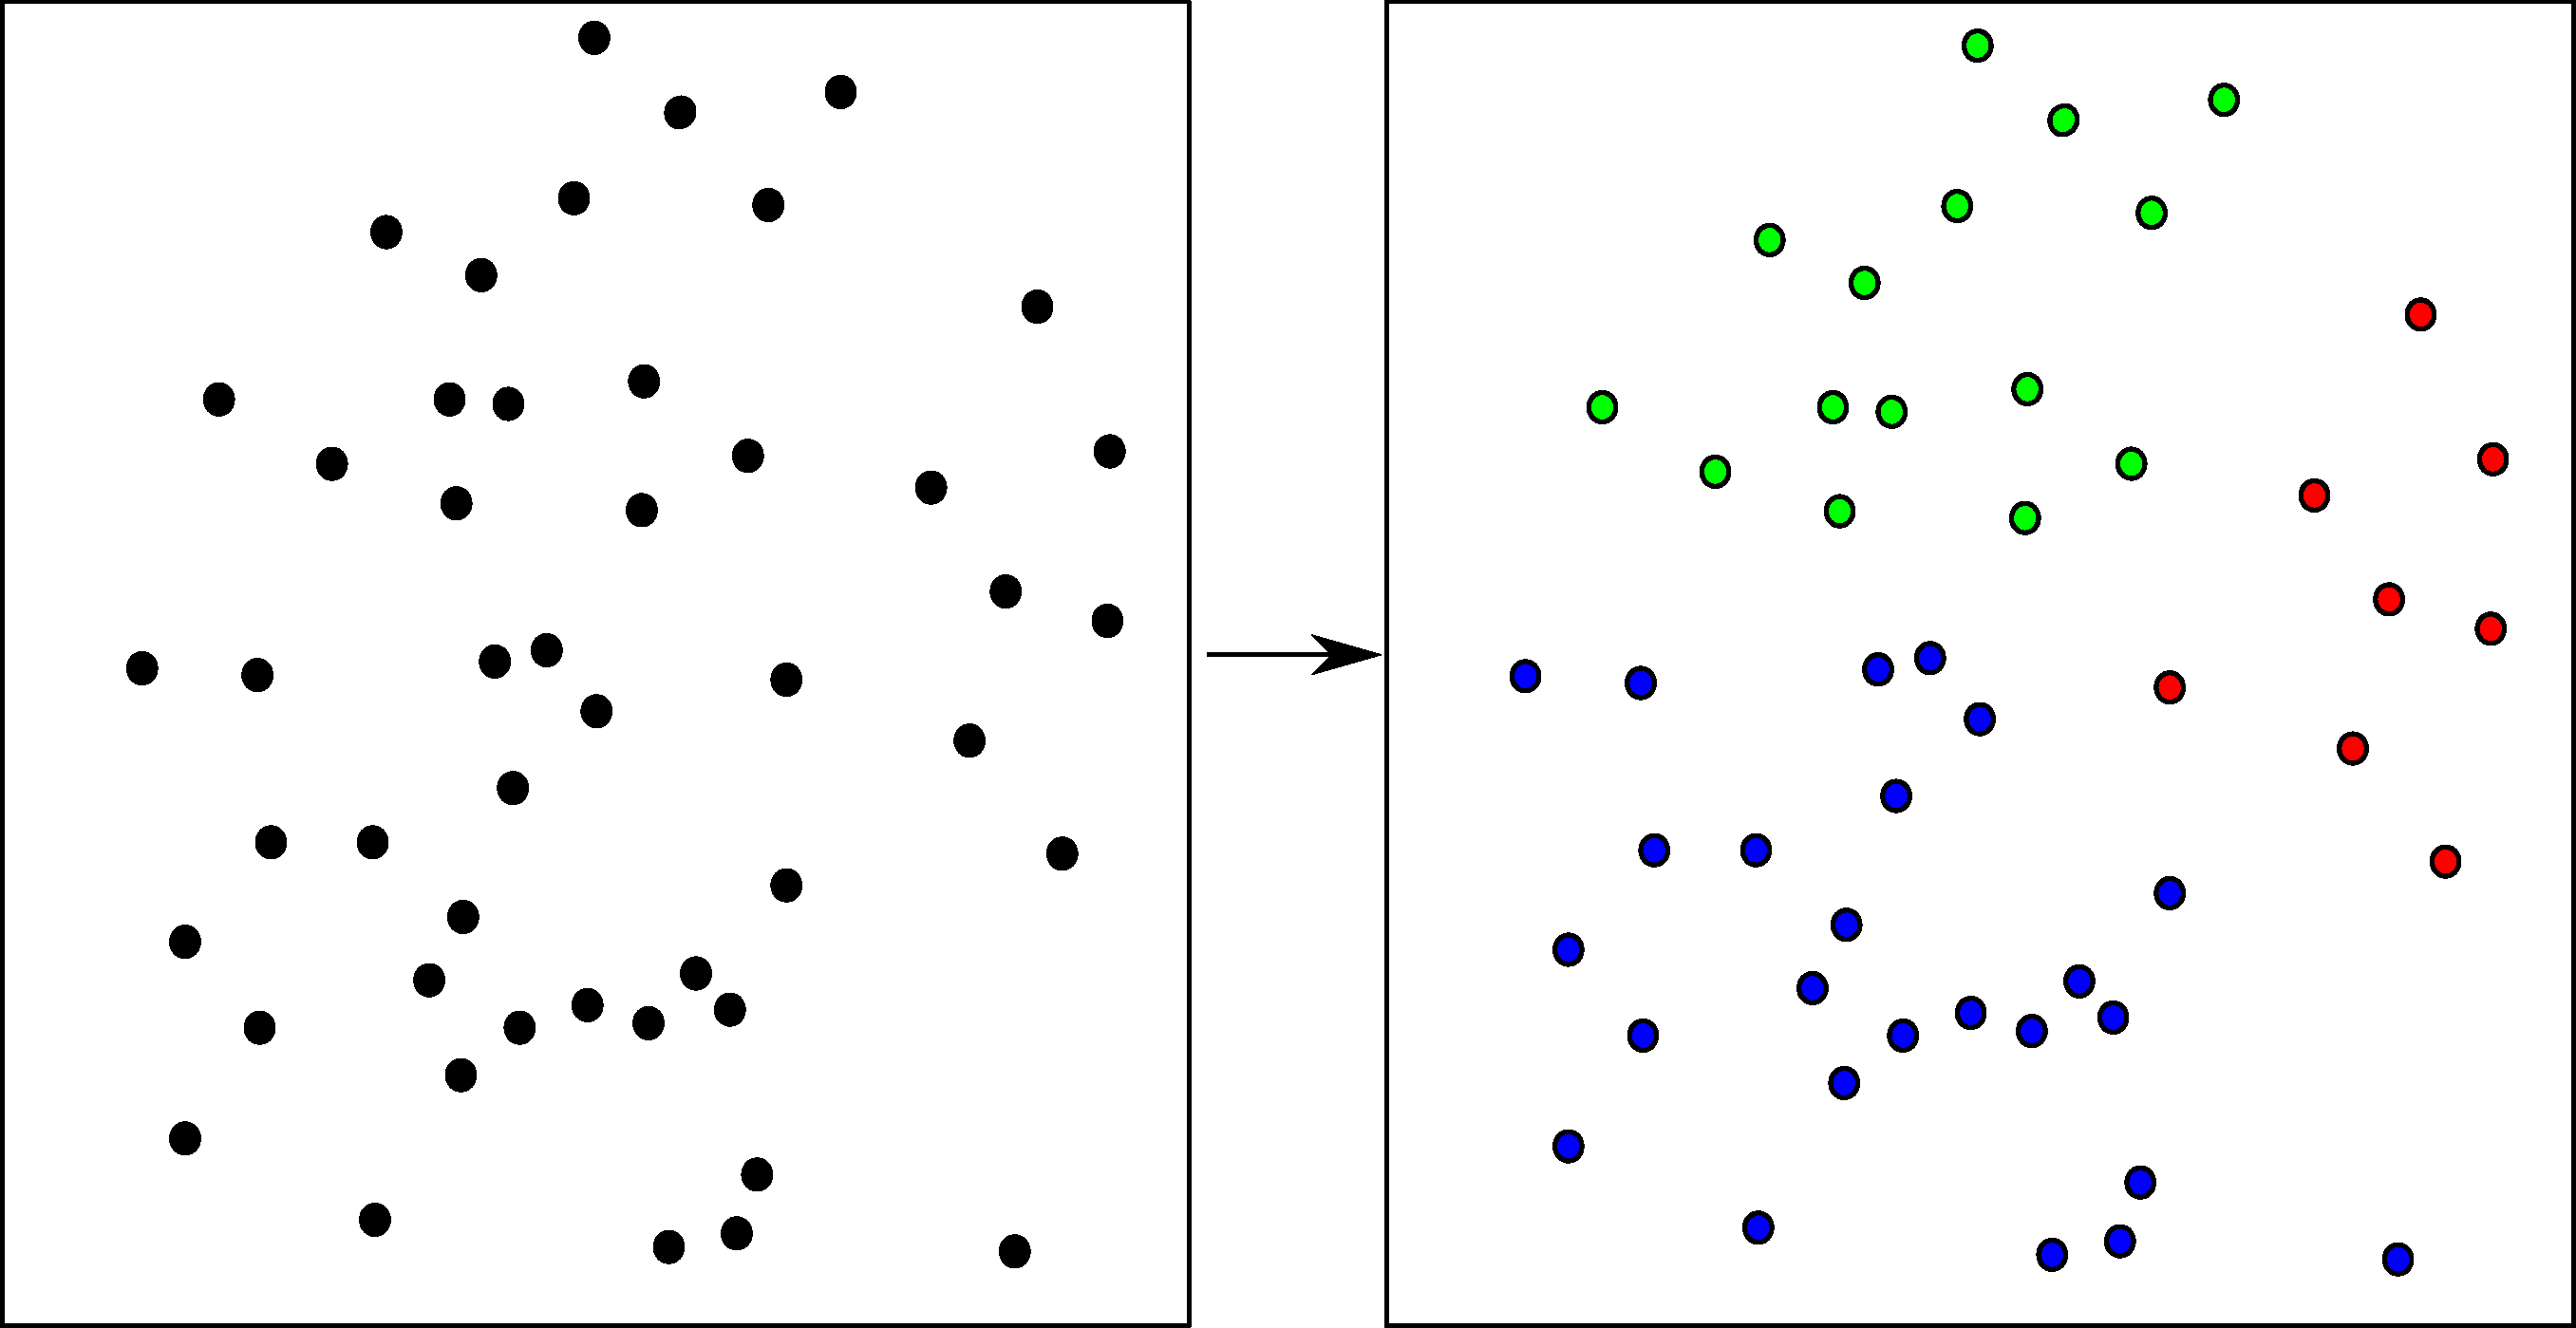
\includegraphics[width=0.45\textwidth]{fig/clustering}
     \hspace{5mm}
     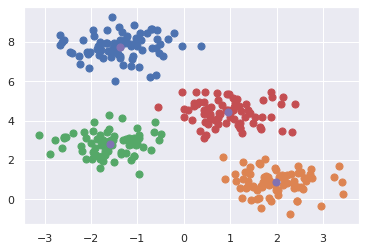
\includegraphics[width=0.45\textwidth]{fig/clustering_done}
    \end{figure}
\end{frame}

\begin{frame}{Very intuitive algorithm}
    What would you do? \pause
    
    \begin{enumerate}
     \item Initialise randomly $K$ centroids.
     \item Assign each data point to the closes centroid.
     \item Recompute centroids from the assignments.
     \item Iterate the past two steps.
    \end{enumerate}\vspace{3mm}
    
    This is called the $K$-means algorithm. Let's see it on colab.
\end{frame}

\begin{frame}{Important points of $K$-means}
 \begin{block}{Automatic inference of latent variables}
  The point-to-cluster assignment variable is \textbf{unknown}/\textbf{latent}/\textbf{hidden}, and must be infered together with the parameters.
 \end{block}

 \begin{block}{Limited to spherical and equally populated clusters}
  The assignment criterion is the Euclidean distances $\Rightarrow$ groups are spherical and equally populated.
 \end{block}
 
 \begin{figure}
  \centering
       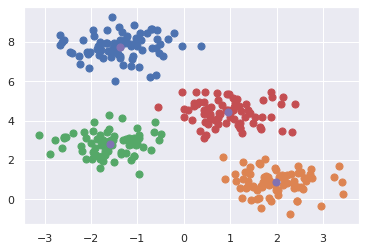
\includegraphics[width=0.45\textwidth]{fig/clustering_done}
     \hspace{5mm}
     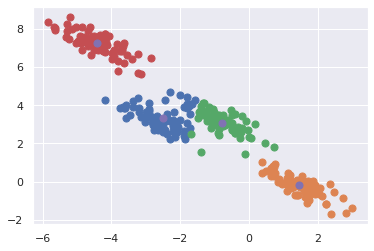
\includegraphics[width=0.45\textwidth]{fig/clustering_fail}
 \end{figure}
\end{frame}

\begin{frame}{Generalising $K$-means: GMM}
\remark{gmm-def}{Gaussian mixture model (GMM):
\begin{itemize}
 \item For each data point $\bs{x}_n$ there is a hidden variable $z_n$ taking discrete values from 1 to $K$: $z_n\in\{1,\ldots,K\}$.\pause
 \item Its prior probability is defined as: $p(z_n=k)=\pi_k$, $\sum_{k=1}^K \pi_k = 1$.\pause
 \item Given $z_n$, the data point is modeled as a multivariate Gaussian:\vspace{-2mm}
 \[p(\bs{x}_n|z_n=k) = \mathcal{N}(\bs{x}_n;\bs{\mu}_k,\bs{\Sigma}_k) \]\vspace{-4mm}
\end{itemize}
}\vspace{3mm}
Advantages:
 \begin{enumerate}
  \item Having $\pi_1,\ldots,\pi_K$ means that groups can be differently populated.
  \item The shape of the groups is modeled by $\bs{\Sigma}_k$.
 \end{enumerate}
\end{frame}

\begin{frame}{Maximum likelihood for GMM}
 Let's compute $p(\bs{x}_n)$
 \[ p(\bs{x}_n) = \sum_{k=1}^K p(\bs{x}_n,z_n=k) = \sum_{k=1}^K \pi_k\mathcal{N}(\bs{x}_n;\bs{\mu}_k,\bs{\Sigma}_k).\]
 The log-likelihood:
 \[\mathcal{L}(\bs{\Theta}|\bs{X}) = \sum_{n=1}^N \log  \sum_{k=1}^K \pi_k\mathcal{N}(\bs{x}_n;\bs{\mu}_k,\bs{\Sigma}_k),\]
 {\small with $\bs{\Theta}=\{\pi_k,\bs{\mu}_k,\bs{\Sigma}_k\}_{k=1}^K$.}\vspace{5mm}\\
 Compute either $\displaystyle\frac{\partial\mathcal{L}}{\partial\pi_k}$, $\displaystyle\frac{\partial\mathcal{L}}{\partial\bs{\mu}_k}$ or $\displaystyle\frac{\partial\mathcal{L}}{\partial\bs{\Sigma}_k}$.\pause\ Very difficult to optimise.
\end{frame}

\section{Maximum Likelihood for GMM: the EM algorithm}

\begin{frame}{Log-likelihood?}
 We have see that $\log p(\bs{x})$ does not work well with derivatives.\vspace{3mm}\\
 
 However, $\log p(\bs{x},z)$ does!\vspace{3mm}\\
 
 Problem: $z$ is not observed, we must take the expectation w.r.t.\ $z$.\vspace{3mm}\\
 \vspace{3mm}\pause

 We propose to do it using the posterior distribution $p(z|\bs{x})$:\\
 {\small (we will justify this choice later on)}
 \[\mathcal{Q}(\bs{\Theta},\bs{\Theta}^0) = \mathbb{E}_{p(z|\bs{x};\bs{\Theta}^0)} \log p(\bs{x},z;\bs{\Theta})\]
 
 This function is called: expected complete-data log-likelihood.
\end{frame}


\begin{frame}{Towards the EM algorithm for GMM}
 Notation: observations $\bs{X}=\{\bs{x}_n\}_{n=1}^N$, latent variables $\bs{Z}=\{z_n\}_{n=1}^N$ and parameters $\bs{\Theta}=\{\pi_k,\bs{\mu}_k,\bs{\Sigma}_k\}_{k=1}^K$.\vspace{4mm}\\\pause
 
 \remark{em-gmm}{Given $\bs{\Theta}^0$, we use the \textit{expected complete-data log-likelihood} $\mathcal{Q}$:\vspace{2mm}
 \begin{enumerate}
  \item Expectation: \vspace{-9mm} 
  \[ \mathcal{Q}(\bs{\Theta},\bs{\Theta}^0) = \mathbb{E}_{p(\bs{Z}|\bs{X};\bs{\Theta}^0)} \log p(\bs{Z},\bs{X};\bs{\Theta})\]\vspace{-5mm}
  \item Maximisation: \vspace{-5mm} 
  \[ \bs{\Theta}^1 = \arg\max_{\bs{\Theta}} \mathcal{Q}(\bs{\Theta},\bs{\Theta}^0)\]
 \end{enumerate}}\pause\vspace{4mm}
 
  We can look back to $K$-means:
 \begin{enumerate}
  \item Infer latent variables (assignment) given the parameters (centroids).
  \item Estimate the parameters (centroids) given the assignments.
 \end{enumerate} 
\end{frame}




\begin{frame}{EM for GMM}
 Let's recall: $p(z_n=k)=\pi_k$ \& $p(\bs{x}_n|z_n=k) = \mathcal{N}(\bs{x}_n;\bs{\mu}_k,\bs{\Sigma}_k)$.\vspace{5mm}\\
 \textbf{Expectation}: Compute $\mathcal{Q}(\bs{\Theta},\bs{\Theta}^0) = \mathbb{E}_{p(\bs{Z}|\bs{X};\bs{\Theta}^0)} \log p(\bs{Z},\bs{X};\bs{\Theta})$.\vspace{2mm}\\
 \begin{itemize}
  \item Start with $p(z_n=k|\bs{x}_n;\bs{\Theta}^0)$.\pause\ And name it $\eta_{nk}=p(z_n=k|\bs{x}_n;\bs{\Theta}^0)$.\\
  \textcolor{red}{$\eta_{nk}$ is the posterior probability that $\bs{x}_n$ belongs to group $k$.}\vspace{2mm}
  \item Then $p(\bs{x}_n,z_n|\bs{\Theta})$\pause$ =\pi_k\mathcal{N}(\bs{x}_n;\bs{\mu}_k,\bs{\Sigma}_k)$.\vspace{2mm}
  \item Also $\mathbb{E}_{p(z_n|\bs{X}_n;\bs{\Theta}^0)} \log p(z_n,\bs{x}_n;\bs{\Theta})$\pause$ =\sum_{k=1}^K \eta_{nk} \log \pi_k\mathcal{N}(\bs{x}_n;\bs{\mu}_k,\bs{\Sigma}_k)$.\vspace{2mm}
 \end{itemize}
\remark{Q-gmm}{  \[\mathcal{Q}(\bs{\Theta},\bs{\Theta}^0) = \sum_{n=1}^N\sum_{k=1}^K \eta_{nk} \log \pi_k\mathcal{N}(\bs{x}_n;\bs{\mu}_k,\bs{\Sigma}_k).\]}

\end{frame}
 
 \begin{frame}{EM for GMM (II)}
  Let's recall:
  \[\mathcal{Q}(\bs{\Theta},\bs{\Theta}^0) = \sum_{n=1}^N\sum_{k=1}^K \eta_{nk} \log \pi_k\mathcal{N}(\bs{x}_n;\bs{\mu}_k,\bs{\Sigma}_k).\]
  This splits:
  \[\mathcal{Q}(\bs{\Theta},\bs{\Theta}^0) = \sum_{n=1}^N\sum_{k=1}^K \eta_{nk} \log \pi_k + \eta_{nk}\log\mathcal{N}(\bs{x}_n;\bs{\mu}_k,\bs{\Sigma}_k).\]
  We consider now the Lagrangian for $\pi_1,\ldots,\pi_K$:
  \[\mathcal{Q}(\bs{\Theta},\bs{\Theta}^0) = \sum_{n=1}^N\sum_{k=1}^K \eta_{nk} \log \pi_k + \beta\Big(1-\sum_{k=1}^K \pi_k\Big).\]
 \end{frame}
 
 \begin{frame}{EM for GMM (III)}
  \exercise{M-step-gmm}{Prove that the optimal parameters write:
  \[\pi_k^* = \frac{1}{N}S_k, \qquad S_k = \sum_{n=1}^N \eta_{nk},\]
  and:
  \[\bs{\mu}_k^*=\frac{1}{S_k}\sum_{n=1}^N\eta_{nk}\bs{x}_n\qquad \bs{\Sigma}_k^* = \frac{1}{S_k}\sum_{n=1}^N\eta_{nk} (\bs{x}_n-\bs{\mu}_k^*)(\bs{x}_n-\bs{\mu}_k^*)^\top.\]}
%   You must prove this as previous work of the Lab session.
 \end{frame}

\section{The EM algorithm}

\begin{frame}{The EM in general}
Let us assume a probabilistic graphical model, with observed variables $\bs{X}$, hidden variables $\bs{z}$ and parameters $\bs{\Theta}$.\vspace{3mm}

\remark{em-general}{
 Initialise the parameters $\bs{\Theta}^0$. For iteration $r=1,\ldots,R$:
 \begin{description}
  \item[E-step] Compute $p(\bs{z}|\bs{X};\bs{\Theta}^{r-1})$ and $\mathcal{Q}(\bs{\Theta},\bs{\Theta}^{r-1})$.
  \item[M-step] Compute $\bs{\Theta}^{r}=\arg\max_{\bs{\Theta}} \mathcal{Q}(\bs{\Theta},\bs{\Theta}^{r-1})$.
 \end{description}
 }\vspace{3mm}

 Comments
\begin{itemize}
 \item EM is sensible to initialisation.
 \item It may converge to a local maxima.
 \item We still need to compute and optimise $\mathcal{Q}(\bs{\Theta},\bs{\Theta}^{r-1})$.
\end{itemize}
\end{frame}

\begin{frame}{But why does it work?}
 The main mathematical object in EM is $\mathcal{Q}$.\\ {\footnotesize (The expected complete-data log-likelihood).}\vspace{4mm}\\
 
 What is the relationship with the log-likelihood?\\ Let's take any distribution of $\bs{z}$: $q(\bs{z})$ and ignore $\bs{\Theta}$ for the time being.
 \begin{align*}
\log p(\bs{x})&= \mathbb{E}_{q(\bs{z})}\Big[\log p(\bs{x})\Big]\\
&= \mathbb{E}_{q(\bs{z})}\Big[\log p(\bs{x})\frac{p(\bs{z}|\bs{x})q(\bs{z})}{p(\bs{z}|\bs{x})q(\bs{z})}\Big]\\
&= \mathbb{E}_{q(\bs{z})}\Big[\log \frac{p(\bs{x})p(\bs{z}|\bs{x})}{q(\bs{z})}\Big] +  D_{\text{KL}}\Big(q(\bs{z})\Big\lVert p(\bs{z}|\bs{x})\Big)
\end{align*}
\end{frame}

\begin{frame}{But why does it work? (II)}
 \begin{align*}
\log p(\bs{x};\bs{\Theta}) &= \underbrace{\mathbb{E}_{q(\bs{z})}\Big[\log \frac{p(\bs{x})p(\bs{z}|\bs{x})}{q(\bs{z})}\Big]}_{\text{M-step}} +  \underbrace{D_{\text{KL}}\Big(q(\bs{z})\Big\lVert p(\bs{z}|\bs{x})\Big)}_{\text{E-step}}
\end{align*}
Another interpretation. Given $\bs{\Theta}^0$:
\begin{enumerate}
 \item Set $q(\bs{z})=p(\bs{z}|\bs{x};\bs{\Theta}^0)$.
 \item Optimise w.r.t.\ $\bs{\Theta}$:\vspace{-3mm}
 \[ \mathbf{E}_{q(\bs{z})} \Big[\log \frac{p(\bs{x},\bs{z};\bs{\Theta})}{q(\bs{z})}\Big] \]
\end{enumerate}
\begin{block}{Why?}
  E-step: reduce the distance between log-likelihood and $\mathcal{Q}$.\\
  M-step: push $\mathcal{Q}$ and therefore push the log-likelihood.
\end{block}
\end{frame}

\begin{frame}{But why does it work? (III)}
\begin{align*}
\log p(\bs{x};\bs{\Theta}) &= \underbrace{\mathbb{E}_{q(\bs{z})}\Big[\log \frac{p(\bs{x})p(\bs{z}|\bs{x})}{q(\bs{z})}\Big]}_{ \mathcal{L}(q,\bs{\Theta}) } +  \underbrace{D_{\text{KL}}\Big(q(\bs{z})\Big\lVert p(\bs{z}|\bs{x})\Big)}_{\textrm{KL}(q\lVert p)}
\end{align*}
 
\begin{figure}
 \centering
 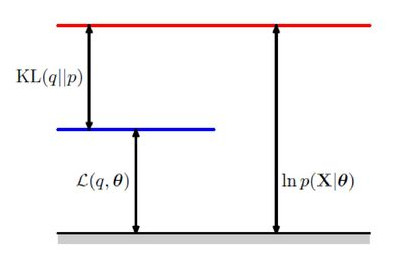
\includegraphics[width=0.4\textwidth]{fig/em-gap.jpg}
\end{figure}

\end{frame}





\end{document}

